\documentclass[11pt]{article}

\usepackage[english]{babel}
\usepackage[utf8]{inputenc}
\usepackage{amsmath}
\usepackage{amsfonts}
\usepackage[ampersand]{easylist}
\usepackage{authblk}
\usepackage{MnSymbol}
\usepackage{graphicx}
\usepackage[colorinlistoftodos]{todonotes}
\usepackage{geometry}
\usepackage{color}
\usepackage{mathtools}
\usepackage{tikz}
\usetikzlibrary{arrows}
\DeclarePairedDelimiter\ceil{\lceil}{\rceil}
\DeclarePairedDelimiter\floor{\lfloor}{\rfloor}

\newcommand{\wh}{\widehat}
\newcommand{\bs}{\boldsymbol}


\geometry{letterpaper}
	\setlength{\oddsidemargin}{0cm}
	\setlength{\evensidemargin}{0cm}
	\setlength{\headheight}{0.5cm}
	\setlength{\headsep}{0cm}
	\setlength{\textwidth}{16cm}
	\setlength{\textheight}{21.0cm}
	\baselineskip=24pt

\title{Applied/Numerical Qualifier Solution: January 2009}

\author{Bennett Clayton}
\affil{Texas A\&M University}
\date{\today}

\begin{document}
\maketitle

{\bf Problem 1.} Let $\Omega = (0,1)$ and $u$ be the solution of the boundary value problem
\begin{align}
    u^{(4)} - (k(x) u')' + q(x) u &= f(x) \label{pb1:eq1} \\
    u(0) = u''(0) &= 0 \\
    u(1) = 0, \quad u''(1) + \beta u'(1) &= \gamma,
\end{align}
for $x \in \Omega$ where $k(x) \geq 0 $, $q(x) \geq 0$, $f(x)$, $\gamma$, and $\beta > 0$ are given data. 

\vskip 1cm

{\bf a.} Derive the weak formulation of this problem.
Specificy the appropriate Sobolev spaces and show that the corresponding bilinear form is coercive.

\vskip 1cm

{\bf Solution}: Let $V := \{v \in H^2(\Omega) : v(0) = v(1) = 0\}$ with the norm $||v||_V := ||v||_{H^2(\Omega)}$.
Then multiply \eqref{pb1:eq1} by $v \in V$ and integrate. 
Doing so, gives us
\begin{align*}
    \int_0^1 u^{(4)}v - (k(x) u')' v + q(x) uv \: dx &= [u'''v]_0^1 - \int_0^1 u'''v' \: dx \\
    &\quad\quad\quad - [k(x)u'v]_0^1 +\int_0^1 k(x) u' v' + q(x) uv \: dx \\
    &= -[u''v']_0^1 + \int_0^1 u'' v'' + k(x) u'v' + q(x) uv \: dx \\
    &= -u''(1)v'(1) + \int_0^1 u'' v'' + k(x) u'v' + q(x) uv \: dx \\
    &= -\gamma v'(1) + \beta u'(1) v'(1)  + \int_0^1 u'' v'' + k(x) u'v' + q(x) uv \: dx 
\end{align*}
Adding $\gamma v'(1)$ to the right hand side with $\int_0^1 f(x) v \: dx$, we define the bilinear and linear forms respectively,
\begin{align}
    a(u,v) &:= \int_0^1 u'' v'' + k(x) u'v' + q(x) uv \: dx + \beta u'(1) v'(1) \\
    F(v) &:= \int_0^1 f(x) v \: dx + \gamma v'(1).
\end{align}
So our weak formulation is: Find $u \in V$ such that for all $v \in V$,
\begin{equation}
    a(u,v) = F(v).
\end{equation}
Note that $u(0) = u(1) = 0$ are essential boundary conditions, whereas $u''(0) = 0$ and $u''(1) + \beta u'(1) = \gamma$ are natural boundary conditions, since they occur ``naturally" in the variational formulation.
Before proving coercivity, we need a Poincar\`{e} inequality.
So consider,
\begin{align*}
    ||u||^2_{L^2(0,1)} &= \int_0^1 u^2 \: dx \\
    &= \int_0^1 \Big( \int_0^x u'(s) \: ds \Big)^2 \: dx \\
    &\leq \int_0^1 x \int_0^x (u'(s))^2 \: ds \: dx \\
    &\leq \int_0^1 (u'(x))^2 \: dx \\
    &= ||u'||^2_{L^2(0,1)}.
\end{align*}
We need one more inequality, so consider,
\begin{align*}
    ||u'||^2_{L^2(0,1)} &= \int_0^1 (u'(x))^2 \: dx \\
    &= \int_0^1 \Big( u'(1) - \int_x^1 u''(s) \: ds \Big)^2 \: dx \\
    &\leq \int_0^1 2(u'(1))^2 + 2\Big( \int_x^1 u''(s) \: ds \Big)^2 \: dx \\
    &\leq 2(u'(1))^2 + 2\int_0^1 (u''(x))^2 \: dx \\
    &= 2(u'(1))^2 + 2||u''||^2_{L^2(0,1)} 
\end{align*}
Now for the coercivity, 
\begin{align*}
    a(u,u) &= \int_0^1 (u'')^2 + k(x) (u')^2 + q(x) u^2 \: dx + \beta (u'(1))^2 \\
    &\geq \tfrac{1}{2} ||u''||^2_{L^2(0,1)} + \tfrac{1}{2} ||u''||^2_{L^2(0,1)} + \beta (u'(1))^2 \\
    &\geq \tfrac{1}{2} ||u''||^2_{L^2(0,1)} + \min\big\{ \tfrac{1}{2}, \beta \big\} \big(||u''||^2_{L^2(0,1)} + (u'(1))^2\big) \\
    &\geq \frac{1}{2}||u''||^2_{L^2(0,1)} + \frac{1}{2}\min\Big\{\frac{1}{2}, \beta \Big\} ||u'||^2_{L^2(0,1)} \\
    &= \frac{1}{2}||u''||^2_{L^2(0,1)} + \frac{1}{4}\min\Big\{\frac{1}{2}, \beta \Big\} ||u'||^2_{L^2(0,1)} + \frac{1}{4}\min\Big\{\frac{1}{2}, \beta \Big\} ||u'||^2_{L^2(0,1)} \\
    &\geq \frac{1}{2}||u''||^2_{L^2(0,1)} + \frac{1}{4}\min\Big\{\frac{1}{2}, \beta \Big\} ||u'||^2_{L^2(0,1)} + \frac{1}{4}\min\Big\{\frac{1}{2}, \beta \Big\} ||u||^2_{L^2(0,1)} \\
    &\geq \frac{1}{4} \min \big\{\frac{1}{2}, \beta \big\} (||u''||^2_{L^2(0,1)} + ||u'||^2_{L^2(0,1)} + ||u||^2_{L^2(0,1)}) \\
    &= \frac{1}{4} \min \big\{\frac{1}{2}, \beta \big\} ||u||^2_{H^2(0,1)}.
\end{align*}



\vskip 2cm



{\bf b.} Suggest a finite element approximation to this problem using piecewise polynomial functions over a uniform partition of $\Omega$ into subintervals with length $h = 1/N$.

\vskip 1cm

{\bf Proof}: We suggest the use of the finite element $(\widehat{K}, \widehat{P}, \widehat{\Sigma})$ where $\widehat{K} = [0,1]$, $\widehat{P} = \mathbb{P}^3[0,1]$ defined on $\widehat{K}$ and $\widehat{\Sigma} = \{\wh{\sigma}_0, \wh{\sigma}_1, \wh{\sigma}_2, \wh{\sigma}_3 \}$ with
\begin{align*}
	\wh{\sigma}_0(f) &:= f(0), \qquad \wh{\sigma}_1(f) := f(1), \\
	\wh{\sigma}_2(f) &:= f'(0), \qquad \wh{\sigma}_3(f) := f'(1),
\end{align*}
for $f \in \widehat{P}$.
The Ciarlet triple, $(\widehat{K}, \widehat{P}, \widehat{\Sigma})$, is indeed a finite element if $\widehat{\Sigma}$ is unisolvent and $\dim(\widehat{P}) = \text{card}(\widehat{\Sigma})$. 
To see that $\widehat{\Sigma}$ is unisolvent for cubic polynomials, one only needs to check for $p\in\widehat{P}$, that if $\wh{\sigma}(p) = 0$ for all $\wh{\sigma} \in \widehat{\Sigma}$ then $p \equiv 0$.
(We leave this proof as an exercise.)
Note that we call this finite element a \textit{Hermite element}.

The shape functions, $\{\widehat{\theta}_j\}_{j\in\{0:3\}}$, for the Ciarlet triple, $(\widehat{K},\widehat{P},\widehat{\Sigma})$, can be found by solving the system of equations $\sigma_i(\widehat{\theta}_j) = \delta_{ij}$ for $i,j \in \{0:3\}$. 
Doing so we find the following: $\widehat{\theta}_0(x) = (x-1)(2x^2 - x - 1)$, $\widehat{\theta}_1(x) = -x^2(2x-3)$, $\widehat{\theta}_2(x) = x(x-1)^2$, $\widehat{\theta}_3(x) = x^2(x-1)$.

Let $K_i := [x_{i-1}, x_i]$ with $x_i - x_{i-1} = h$ for $i \in \{1:N\}$ be our uniform partion of $\Omega$ with the corresponding affine geometric mappings, $T_{K_i} : \widehat{K} \to K_i$. 
Then define $\mathcal{T}_h := \{K_i\}_{i\in\{1:N\}}$ to be our sequence of shapes (our mesh) with the corresponding finite element approximation space,
\begin{equation}
	P(\mathcal{T}_h) := \{ v \in C^1(\Omega) : v|_K \circ T_K \in \widehat{P}, \forall K \in \mathcal{T}_h, v(0) = v(1) = 0 \}.
\end{equation}

The global shape functions can be constructed for $P(\mathcal{T}_h)$, by using the global linear functionals $\sigma_i$ and $\sigma_i'$ defined by $\sigma_i(f) := f(x_i)$ and $\sigma_i'(f) := f'(x_i)$ for $i \in \{0:N\}$.
Specifically, for $i \in \{1, N-1\}$, we have $\phi_i|_{K_i} = \widehat{\theta}_1 \circ T^{-1}_{K_i}$, $\phi_i|_{K_{i+1}} = \widehat{\theta}_0\circ T^{-1}_{K_{i+1}}$ and $\phi_i|_{K_j} = 0$ for $j \neq i, i+1$.
Also, $\psi_i$ can be defined similarly with $\widehat{\theta}_2$ and $\widehat{\theta}_3$.
For a more concrete demonstration, we present the basis functions exaclty,
\begin{align}
    \psi_i(x) &= \begin{cases}
    \frac{1}{h^2}(x - x_i)(x - x_{i-1})^2 &\quad \text{ for } x \in [x_{i-1}, x_i], \\
    \frac{1}{h^2} (x - x_{i+1})^2(x - x_i) &\quad \text{ for } x \in [x_i, x_{i+1}], \\
	    0 &\quad \text{ otherwise},
    \end{cases} \\
    \phi_i(x) &= \begin{cases}
    \frac{1}{h^2}(x - x_{i-1})^2 \big(\frac{2}{h}(x_i - x) + 1\big) &\quad \text{ for } x \in [x_{i-1},x_i], \\
    \frac{1}{h^2}(x_{i+1}-x)^2 \big( \frac{2}{h}(x - x_i) + 1 \big) &\quad \text{ for } x \in [x_i, x_{i+1}], \\
    0 &\quad \text{ otherwise}.
    \end{cases} 
\end{align}
It turns out that these global shape functions form a basis for this space.
That is, $P(\mathcal{T_h}) = \text{span}\big(\{\phi_i\}_{i=1}^{N-1}, \{\psi_i\}_{i=0}^N \big)$. 
(Note: $\phi_i$ and $\psi_i$ are called the cubic Hermite polynomials, not to be confused with the cubic Hermite spline.)

$\blacksquare$



\vskip 2cm




{\bf c.} Derive an error estimate for the finite element solution.

\vskip 1cm

{\bf Proof}: Assume our solution, $u$, is smooth enough; that is, let $u \in H^4(\Omega)$.
Let $\Pi_h :C^1(\Omega) \to V_h$ be the canonical interpolation operator that projects onto our finite dimensional subspace. 
That is,
\begin{equation}
    (\Pi_h u)(x) = \sum_{i=1}^{N-1} \sigma_i(u) \phi_i(x) + \sum_{i=0}^N \sigma_i'(u) \psi_i(x).
\end{equation}
Since $a(\cdot, \cdot)$ is continuous and coercive and our problem has a unique solution by Lax-Milgram, we can apply Cea's lemma.
So we have,
\begin{equation}
    ||u - u_h||_{H^2(\Omega)} \leq C \inf_{v_h \in V_h} ||u - v_h||_{H^2(\Omega)} \leq ||u - \Pi_h u||_{H^2(\Omega)}.
\end{equation}
We perform the usual analysis by transforming to the reference element.
We let $T_{K_i} : [0,1] \to K_i$, defined by 
\begin{equation}
    x = T_{K_i}(\hat{x}) = \hat{x} h + x_{i-1},
\end{equation}
and the inverse transformation is defined similarly,
\begin{equation}
    \hat{x} = T_{K_i}^{-1}(x) = \frac{x - x_{i-1}}{h}.
\end{equation}
We now perform the usual analysis by transforming to the reference element and then applying the Bramble-Hilbert lemma.
Thus, we have the following,
\begin{align*}
    ||u - \Pi_h u||^2_{H^2(\Omega)} &= \sum_{i = 1}^N ||u - \Pi_h u||^2_{H^2([x_{i-1},x_i])} \\
    &= \sum_{i=1}^N \int_{x_{i-1}}^{x_i} | u_i(x) - (\Pi_h u)_i(x) |^2 + |u_i'(x) - (\Pi_h u)_i'(x)|^2 + |u_i''(x) - (\Pi_h u)_i''(x)|^2 \: dx \\
    &= \sum_{i=1}^N \int_0^1 \big( | u_i(T_{K_i}(\hat{x})) - (\Pi_h u)_i(T_{K_i}(\hat{x})) |^2 + |u_i'(T_{K_i}(\hat{x})) - (\Pi_h u)_i'(T_{K_i}(\hat{x}))|^2 \\
    &\qquad\qquad + |u_i''(T_{K_i}(\hat{x})) - (\Pi_h u)_i''(T_{K_i}(\hat{x}))|^2 \big) \: h d\hat{x},
\end{align*}
where the subscript $i$ represents the restriction of the function to the interval $K_i$.
(Note that is it not entirely necessary to consider the restriction to the element $K_i$ since the mapping $T_{K_i}$ will automatically stay on the element $K_i$.
However, we do so merely to keep track of what's going on in the computations.)

Before continuing further we need to discuss the projection operator $\Pi_h$ in more detail.
We start by letting $\widehat{
\Pi} : C^1(\wh{K}) \to \wh{P}$ and $\Pi_{h,i} : C^1(K_i) \to P$, defined in a similar way as $\Pi_h$, where $P = \wh{P} \circ T^{-1}_{K_i}$; that is, $p \in P$ if an only if there exists $\hat{p} \in \wh{P}$ such that $p = \hat{p} \circ T_{K_i}^{-1}$.
We can observe the relationships of these projections through the following diagram where $\psi$ is the \textit{pullback} operator defined as $\psi(v) = v \circ T_{K_i}$,
\begin{center}
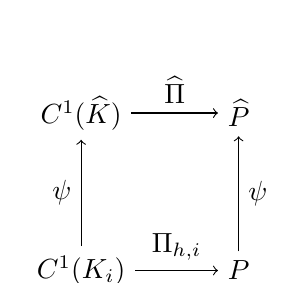
\begin{tikzpicture}
    \node (r) at (0,0) {$C^1(\wh{K})$};
    \node (k) at (2,0) {$\wh{P}$};
    \node (q) at (2,-2) {$P$};
    \node (ra) at (0,-2) {$C^1(K_i)$};
    \draw[->] (ra)--(r) node[midway,left] {$\psi$};
    \draw[->] (r)--(k) node[midway,above] {$\widehat{\Pi}$};
    \draw[->] (ra)--(q) node[midway, above] {$\Pi_{h,i}$};
    \draw[->] (q)--(k) node[midway,right] {$\psi$};
\end{tikzpicture}
\end{center}
Note also that, $(\Pi_h u) \circ T_{K_i} \in \wh{P}$ and $(\Pi_h u)|_{K_i} \circ T_{K_i} = \Pi_{h,i}(u|_{K_i}) \circ T_{K_i}$.
From the diagram, it is easy to see that 
\begin{equation}
    \Pi_{h,i}(u|_{K_i}) \circ T_{K_i} = \widehat{\Pi}(u|_{K_i} \circ T_{K_i}).
\end{equation}
Using this identity, we are able to transform the interpolation operator from $\Pi_h$ to $\widehat{\Pi}$.
In order to simplify notation, we write $\widehat{f_i} := f\circ T_{K_i}$ for $f : K_i \to \mathbb{R}$.
So we have,
\begin{align*}
    ||u - \Pi_h u||^2_{H^2(\Omega)} &= \sum_{i=1}^N \int_0^1 \big( |\widehat{u}_i - \widehat{\Pi} \widehat{u}_i|^2 + \frac{1}{h^2}|\widehat{u}_i' - \widehat{\Pi} \widehat{u}_i'|^2 + \frac{1}{h^4}|\widehat{u}_i'' - \widehat{\Pi} \widehat{u}_i''|^2 \big) h \: d\hat{x} \\
    &= \sum_{i=1}^N \Big( h ||\widehat{u}_i - \widehat{\Pi} \widehat{u}_i||^2_{L^2([0,1])} + \frac{h}{h^2}||\widehat{u}'_i - (\widehat{\Pi} \widehat{u}_i)'||^2_{L^2([0,1])} \\
    &\qquad\qquad + \frac{h}{h^4}||\widehat{u}_i'' - (\widehat{\Pi} \widehat{u}_i)''||^2_{L^2([0,1])} \Big). \\
\end{align*}
Note that $||(\text{Id} - \wh{\Pi})(\cdot)||_{L^2([0,1])}$, $|(\text{Id} - \wh{\Pi})(\cdot)|_{H^1([0,1])}$, and $|(\text{Id} - \wh{\Pi})(\cdot)|_{H^2([0,1])}$ are all bounded sublinear functionals defined on $H^4([0,1])$ which are zero for all $p \in \wh{P}$.
Therefore, we can apply the Bramble-Hilbert lemma to get,
\begin{align*}
    ||u - \Pi_h u||^2_{H^2(\Omega)} &\leq C \sum_{i=1}^N \Big( h |\widehat{u}_i|^2_{H^4([0,1])} + \frac{h}{h^2} |\widehat{u}_i|^2_{H^4([0,1])} + \frac{h}{h^4} |\widehat{u}_i|^2_{H^4([0,1])} \Big) \\
    &= C \sum_{i=1}^N \int_0^1 \Big( \Big| \frac{d^4}{d\hat{x}^4}\widehat{u}_i \Big|^2 + \frac{1}{h^2}\Big| \frac{d^4}{d\hat{x}^4}\widehat{u}_i\Big|^2 +  \frac{1}{h^4}\Big| \frac{d^4}{d\hat{x}^4}\widehat{u}_i \Big|^2 \Big) h \: d\hat{x} \\ 
    &= C\sum_{i=1}^N  \int_{x_{i-1}}^{x_i} h^8 \Big|\frac{d^4}{dx^4} u_i \Big|^2 + h^6 \Big|\frac{d^4}{dx^4}u_i \Big|^2 + h^4 \Big| \frac{d^4}{dx^4} u_i \Big|^2 \: dx \\
    &= C (h^8 + h^6 + h^4) |u|^2_{H^4(\Omega)} \\
    &\leq Ch^4 |u|^2_{H^4(\Omega)}.
\end{align*}
Taking the square root of both sides, we arrive out our error estimate,
\begin{equation*}
    ||u - u_h||_{H^2(\Omega)} \leq Ch^2 |u|_{H^4(\Omega)}.
\end{equation*}
$\blacksquare$


\vskip 2cm





\textbf{Problem 2.} Let $\Omega = (0,1)^2$ and $u$ be the solution of the second order elliptic problem:
\begin{align}
	-\Delta u := -u_{x_1 x_1} - u_{x_2 x_2} &= f(x), \quad \text{ for } x\in \Omega \label{pb2_eq1} \\
    \frac{\partial u}{\partial n} + u &= g(x), \quad \text{ for } x\in\partial\Omega
\end{align}
where $n$ is the outward normal unit vector to the boundary $\partial \Omega$ and $f(x)$ and $g(x)$ are given functions.

\vskip 1cm

\textbf{a.} Derive the weak formulation of this problem in the form $a(u,v) = F(v)$, where $a(u,v)$ and $F(v)$ are the appropriate bilinear and linear forms defined on the Sobolev space $H^1(\Omega)$.

\vskip 1cm

\textbf{Proof:} Multiply \eqref{pb2_eq1} by a test function $v$ in some space $V$ and integrate by parts,
\begin{align*}
    -\int_\Omega \Delta u v \: dx &= \int_\Omega \nabla u \cdot \nabla v \: dx - \int_{\partial\Omega} \frac{\partial u}{\partial n} v \: ds \\
    &= \int_\Omega \nabla u \cdot \nabla v \: dx - \int_{\partial \Omega} g(x) v \: ds + \int_{\partial\Omega} u v \: ds.
\end{align*}
Adding the integral $\int_{\partial \Omega} g(x) v \: ds $ to the right hand side, we have the following bilinear and linear forms,
\begin{align*}
    a(u,v) &= \int_{\Omega} \nabla u \cdot \nabla v \: dx + \int_{\partial\Omega} uv \: ds \\
    F(v) &= \int_\Omega f v \: dx + \int_{\partial\Omega} g v \: ds.
\end{align*}
So the weak formulation of the problem is, find $u \in H^1(\Omega)$ such that $a(u,v) = F(v)$ for all $v \in H^1(\Omega)$.


\vskip 2cm


\textbf{b.} Let $S_h$ be a finite element space of continuous piece-wise polynomial functions defined over a regular partitioning of $\Omega$ into triangles and let $a_h(u, v)$ and $F_h(v)$ be the bilinear forms where all integrals are computed approximately. 
Derive Strang’s lemma for the error of the FEM: find $u_h \in S_h$ such that $a_h(u_h, v) = F_h(v)$, $\forall v \in S_h$.

\vskip 1cm

\textbf{Proof:} Strang's First Lemma: Let $V_h \subset V$ and let the bilinear form $a_h(\cdot, \cdot)$ be uniformly $V_h$-elliptic.
Then there exists a constant $c > 0$ such that 
\begin{equation*}
    ||u - u_h|| \leq c \Big[ \inf_{z_h \in V_h} \big\{ ||u - z_h|| + ||a(z_h, \cdot) - a_h(z_h, \cdot) ||_{*,h} \big\} + ||F - F_h||_{*,h} \Big].
\end{equation*}

To prove this, consider for $z_h, v_h \in V_h$,
\begin{align*}
    a_h(u_h - z_h, v_h) &= a_h(u_h, v_h) - a_h(z_h, v_h) \\
    &= F_h(v_h) - a_h(z_h, v_h) \\
    &= F_h(v_h) - a_h(z_h, v_h) + (a(u,v_h) - F(v_h)) + (a(z_h, v_h) - a(z_h, v_h)) \\
    &= a(u - z_h, v_h) + a(z_h, v_h) - a_h(z_h, v_h) + F_h(v_h) - F(v_h).
\end{align*}
Now we set $v_h = u_h - z_h$ and invoke $V$-ellipticity and continuity of $a$,
\begin{equation*}
    \alpha ||u_h - z_h||^2 \leq ||u - z_h|| ||u_h - z_h|| + |a(z_h, v_h) - a_h(z_h, v_h)| + |F_h(v_h) - F(v_h)|.
\end{equation*}
We can then divide by $||u_h - z_h|| = ||v_h||$, the constant $\alpha$, and then take the supremum over all $v_h \in V_h$ to get,
\begin{equation*}
    ||u_h - z_h|| \leq C ( ||u - z_h|| + ||a(z_h, \cdot) - a_h(z_h, \cdot)||_{*,h} + ||F_h(\cdot) - F(\cdot)||_{*,h}).
\end{equation*}
By the triangle inequality,
\begin{equation*}
    ||u - u_h|| \leq ||u - z_h|| + ||u_h - z_h||.
\end{equation*}
Combining these two, we can then take the infimum over all $z_h$ to get the result.
$\blacksquare$



\vskip 2cm

\textbf{c.}  Let $S_h$ be the finite element space of piece-wise linear functions.
Let all integrals in $a(u, v)$ and $F(v)$ be computed using quadratures. 
Namely, for $\tau$ and $e$ being triangle and edge defined by the vertexes $P_1$, $P_2$, $P_3$ and $P_1$, $P_2$, respectively,
\begin{align}
    \int_\tau w(x) \: dx &\approx \frac{|\tau|}{3}(w(P_1) + w(P_2) + w(P_3)), \\
    \int_e w(x) \: ds &\approx \frac{|e|}{2}(w(\alpha) + w(\beta))
\end{align}
where $|\tau|$ is the area of $\tau$ and $|e|$ is the length of $e$, and $\alpha$ and $\beta$ are the Gaussian quadrature nodes.
Explain why $a(w, v) = a_h(w, v)$ for all $w, v \in S_h$.

\vskip 1cm


\textbf{Proof:} Since $w, v \in S_h$ we have that $\nabla w \cdot \nabla v$ is just a piecewise constant function.
Note that the derivatives on $\Omega$ are assumed to be weak derivatives since $v$ and $w$ are only piecewise linear. 
Once we discretize the domain, we will then view the derivatives in the classical sense as $v$ and $w$ are continuous on each element individually.
Therefore, 
\begin{align*}
    \int_\Omega \nabla w \cdot \nabla v \: dx &= \sum_{\tau \in \mathcal{T}_h} \int_\tau \nabla w \cdot \nabla v \: dx \\
	&= \sum_{\tau \in \mathcal{T}_h} |\tau| \nabla(w|_\tau) \cdot \nabla (v|_\tau) \\
	&= \sum_{\tau \in \mathcal{T}_h} \frac{|\tau|}{3} ((\nabla w \cdot \nabla v)(P_1) + (\nabla w \cdot \nabla v)(P_2) + (\nabla w \cdot \nabla v)(P_3)).
\end{align*}
For the boundary integral, let $\mathcal{F}$ denote the collection of faces of the triangulation $\mathcal{T}_h$.
Denote $\mathcal{F}^\partial := \{ e \in \mathcal{F} : e \subset \partial \Omega \}$.
Next, note that $wv$ is a quadratic one dimensional polynomial. 
The quadrature points are taken to be the Gaussian quadrature, which are exact for polynomials of degree $2n-1$, where $n$ is the number of points used; $n=2$ in our case.
Specifically,
\begin{equation*}
	\int_{\partial \Omega} w v \: ds = \sum_{e \in \mathcal{F}^\partial} \int_e w v \: dx = \sum_{e \in \mathcal{F}^\partial} \int_{-1}^1 (w \circ T_e)(t) (v\circ T_e)(t) \frac{|e|}{2} \: dt = \sum_{e\in\partial\Omega} \frac{|e|}{2}((\hat{w}\hat{v})(\alpha) + (\hat{w}\hat{v})(\beta)),
\end{equation*}
where $T_e : [-1,1] \to e$ and $\hat{w} = w \circ T_e$.
Recall that the Guassian quadrature is defined on the interval $[-1,1]$.
Also, if $e = [a,b]$, the transformation is,
\begin{equation*}
    T(t) = \frac{1}{2}(1-t)a + \frac{1}{2}(t + 1) b.
\end{equation*}
Whence $T'(t) = (b-a)/2 = |e|/2$. 
Thus from the above identities, we have $a_h(w,v) = a(w,v)$ for all $w, v \in S_h$.
$\blacksquare$


\vskip 2cm


\textbf{d.} Using the estimate of Part (b) estimate the error $||u - u_h||_{H^1}$.

\vskip 1cm


\textbf{Proof:} Recall that $a$ is uniformly $H^1$-elliptic, but $a = a_h$ on $S_h\times S_h$, hence $a_h$ is uniformly $S_h$-elliptic.
Because of this, we can apply Strang's lemma, and since $a_h(w,v) = a(w,v)$ for all $w,v \in S_h$, our inequality reduces to,
\begin{equation*}
    ||u - u_h||_{H^1(\Omega)} \leq \inf_{z_h \in S_h} ||u - z_h||_{H^1(\Omega)} + ||f(\cdot) - f_h(\cdot)||_{*,h}.
\end{equation*}
Lets start with $\inf ||u - z_h||_{H^1}$.
Let $\Pi_h$ be the projection onto the space $S_h$, so we have,
\begin{equation*}
    \big(\inf_{z_h \in S_h} ||u - z_h||_{H^1(\Omega)}\big)^2 \leq ||u - \Pi_h u ||_{H^1(\Omega)}^2 = \sum_{\tau \in \mathcal{T}_h} ||u - \Pi_h u||^2_{H^1(\tau)}.
\end{equation*}
Now we transform to the reference element and apply the Bramble-Hilbert lemma.
We also will use the affine geometric mappings $F_\tau : \Hat{\tau} \to \tau$, defined as $F_\tau(\Hat{\bs{x}}) = \mathsf{B}\Hat{\bs{x}} + \bs{b}$, where $\Hat{\tau}$ is the reference element.
Let $F'_\tau$ denote the Jacobian of $F_\tau$ then $|\det(F'_\tau)| = |\tau|/|\Hat{\tau}|$.
Additionally, we skip over the same arguments made about the interpolation operator $\Pi_h$ in Problem 1. c.
So we have,
\begin{align*}
	\sum_{\tau \in \mathcal{T}_h} ||u - \Pi_h u||^2_{H^1(\tau)} &= \sum_{\tau \in \mathcal{T}_h} \int_{\tau} |u - \Pi_h u|^2 + |\nabla(u - \Pi_h u)|^2 \: d\bs{x} \\
	&= \sum_{\tau \in \mathcal{T}_h} \int_{\Hat{\tau}} \Big( |u\circ F_\tau  - \widehat{\Pi} (u\circ F_\tau) |^2 + \Big| \big(\Hat{\nabla} (u\circ F_\tau - \widehat{\Pi}(u\circ F_\tau))\big)^T \mathsf{B}^{-1} \Big|^2 \Big) \frac{|\tau|}{|\Hat{\tau}|} \: d\Hat{\bs{x}},
\end{align*}
where $\hat{\nabla}$ is the gradient with respect to the variables $\hat{\bs{x}} = (\hat{x},\hat{y})$.
We use the inequality, $|\boldsymbol{v}^T A| \leq ||A|||v|$, where $\boldsymbol{v}$ is a vector and $A$ is a matrix; $||\cdot||$ is some matrix norm for $A$. 
Based on the definition of $\mathsf{B}$ (hence $\mathsf{B}^{-1}$) we have that $||\mathsf{B}^{-1}|| \leq C/h$ for some constant $C$.
Using the notation $\hat{u}_\tau := u \circ F_\tau$, we have the following,
\begin{align*}
	\sum_{\tau \in \mathcal{T}_h} ||u - \Pi_h u||^2_{H^1(\tau)} &\leq Ch^2 \sum_{\tau \in \mathcal{T}_h} \int_{\Hat{\tau}} |\hat{u}_\tau - \widehat{\Pi}(\hat{u}_\tau)|^2 \: d\Hat{\bs{x}} + C \sum_{\tau \in \mathcal{T}_h} \int_{\Hat{\tau}} |\Hat{\nabla}(\hat{u}_\tau - \widehat{\Pi}(\hat{u}_\tau))|^2 \: d\Hat{\bs{x}} \\
	&= Ch^2 \sum_{\tau \in \mathcal{T}_h} ||(\text{Id} - \widehat{\Pi})(\hat{u}_\tau)||^2_{L^2(\Hat{\tau})} + C \sum_{\tau \in \mathcal{T}_h} |(\text{Id} - \widehat{\Pi})(\hat{u}_\tau)|^2_{H^1(\Hat{\tau})},
\end{align*}
Notice that $||(\text{Id} - \widehat{\Pi})(\cdot)||_{L^2(\hat{\tau})}$ and $|(\text{Id} - \Hat{\Pi}_h)(\cdot)|_{H^1(\hat{\tau})}$ are both bounded sublinear functionals defined on $H^2(\Hat{\tau})$ and are exactly zero for linear polynomials on $\hat{\tau}$, therefore the Bramble-Hilbert lemma can be applied,
\begin{align*}
    \sum_{\tau \in \mathcal{T}_h} ||u - \Pi_h u||^2_{H^1(\tau)} &\leq Ch^2 \sum_{\tau \in \mathcal{T}_h} |\hat{u}_\tau|^2_{H^2(\Hat{\tau})} + C \sum_{\tau \in \mathcal{T}_h} |\hat{u}_\tau|^2_{H^2(\Hat{\tau})} \\
	&\leq C (h^2 + 1) \sum_{\tau \in \mathcal{T}_h}  \int_{\Hat{\tau}} \sum_{|\alpha| = 2} |\Hat{D}^\alpha \Hat{u}_\tau|^2 \: d\Hat{\bs{x}} \\
	&\leq C \sum_{\tau \in \mathcal{T}_h}  \int_{\tau} \sum_{|\alpha| = 2} ||\mathsf{B}||^4 \big|  D^\alpha u \big|^2 \frac{|\Hat{\tau}|}{|\tau|} \: d\bs{x} \\
	&\leq C \sum_{\tau \in \mathcal{T}_h}  \int_\tau h^2  \sum_{|\alpha|=2} |D^\alpha u|^2 \: d\bs{x} \\
    &= C h^2 |u|^2_{H^2(\Omega)}.
\end{align*}
Thus taking the square root of both sides, we have,
\begin{equation*}
	\inf_{z_h \in S_h} ||u - z_h||_{H^1(\Omega)} \leq Ch |u|_{H^2(\Omega)}.
\end{equation*}

Now for $||F(\cdot) - F_h(\cdot)||_{*,h}$.
To simplify notation we define the following functionals,
\begin{align*}
    E_h(z) &:= \int_\Omega z(x) \: dx - \sum_{\tau \in \mathcal{T}_h} \frac{|\tau|}{3}\sum_{i=1}^3 z(P_i) \\
	G_h(z) &:= \int_{\partial \Omega} z \: ds - \sum_{e \in \mathcal{F}^\partial} \frac{|e|}{2} (z(\alpha) + z(\beta)),
\end{align*}
where $\mathcal{F}$ denotes the collection of all faces of the triangulation $\mathcal{T}_h$, with $\mathcal{F}^\partial$ being the subset of faces belonging to the boundary.
Note that $E_h : H^1(\Omega) \to \mathbb{R}$ is linear, bounded, and the quadrature rule is exact for constant functions.
So $E_h(p) = 0$ for all $p \in \mathbb{P}_0$. 
The strategy is to map to the reference element and then apply the Bramble-Hilbert lemma.
(Remember that the constant in the Bramble-Hilbert lemma depends on the domain, this is why we first map to the reference element.)
So consider,
\begin{align*}
    |E_h(f v_h)| &\leq \sum_{\tau \in \mathcal{T}_h} \Big| \int_\tau f v_h \: dx - \frac{|\tau|}{3} \sum_{i=1}^3 f(P_i) v_h(P_i) \Big| \\
	&= \sum_{\tau \in \mathcal{T}_h}  \frac{|\tau|}{|\Hat{\tau}|} \Big| \int_{\Hat{\tau}} (fv_h)\circ F_\tau \: d\Hat{\bs{x}}  - \frac{|\Hat{\tau}|}{3} \sum_{i=1}^3 (f\circ F_\tau)(\Hat{P}_i) (v\circ F_\tau)(\Hat{P}_i) \Big| \\
    &\leq Ch^2 \sum_{\tau \in \mathcal{T}_h} |(fv_h)\circ F_\tau|_{H^1(\Hat{\tau})} \\
	&\leq Ch^2 \sum_{\tau \in \mathcal{T}_h} \Big( \int_{\tau} h^2 |\nabla(f v_h)|^2 \frac{|\Hat{\tau}|}{|\tau|} \: d\bs{x} \Big)^{1/2} \\
    &\leq Ch^2 \sum_{\tau \in \mathcal{T}_h} |f v_h|_{H^1(\tau)}.
\end{align*}
If we specifically look at the the $H^1$ semi-norm, we can apply the product rule and some other inequalities,
\begin{align*}
    |f v_h|^2_{H^1(\tau)} &= \int_{\tau} |\nabla(f v_h)|^2 \: dx \\
    &= \int_{\tau} |f \nabla v_h + v_h \nabla f|^2 \: dx \\
    &\leq C (||f||^2_{L^\infty(\tau)} |v_h|^2_{H^1(\tau)} + ||\nabla f||^2_{L^\infty(\tau)} ||v_h||^2_{L^2(\tau)}) \\
    &\leq C ||f||^2_{W^{1,\infty}(\tau)} ||v_h||^2_{H^1(\tau)}.
\end{align*}
Taking the square root we have,
\begin{equation*}
    |f v_h|_{H^1(\tau)} \leq C ||f||_{W^{1,\infty}(\tau)} ||v_h||_{H^1(\tau)}.
\end{equation*}
Using this result and some similar arguments from the beginning of the problem, we have,
\begin{align*}
    |E_h(f v_h)| &\leq Ch^2 \sum_{\tau \in \mathcal{T}_h} ||f||_{W^{1,\infty}(\tau)} ||v_h||_{H^1(\tau)} \\
    &\leq Ch^2 ||f||_{W^{1,\infty}(\Omega)} \sum_{\tau \in \mathcal{T}_h} ||v_h||_{H^1(\tau)} \\
    &\leq Ch^2 ||f||_{W^{1,\infty}(\Omega)} \Big( \sum_{\tau \in \mathcal{T}_H} 1^2 \Big)^{1/2} \Big( \sum_{\tau \in \mathcal{T}_H} ||v_h||^2_{H^1(\tau)} \Big)^{1/2} \\
    &= Ch^2 ||f||_{W^{1,\infty}(\Omega)} \sqrt{|\mathcal{T}_h|} ||v_h||_{H^1(\Omega)}.
\end{align*}
Where $|\mathcal{T}_h|$ denotes the number of elements in $\mathcal{T}_h$.
Assuming some shape regularity, we have that $|\mathcal{T}_h| \propto |\Omega|/h^2$. 
Therefore, we can say that,
\begin{equation}
    |E_h(f v_h)| \leq Ch ||f||_{W^{1,\infty}(\Omega)}||v_h||_{H^1(\Omega)}. 
\end{equation}

Now for $G_h$, let $z \in H^1(\Omega)$ which is continuous on $\partial \Omega$ and define $F_e : \hat{e} \to e$ to be the affine transformation of the reference edge $\hat{e}$ to the edge $e$ of an element $\tau$.
Note also that $|\det (F'_e)| = |e|/|\hat{e}|$.
So we have the following,
\begin{align*}
    |G_h(z)| &= \Big| \int_{\partial \Omega} z \: ds - \sum_{e \in \mathcal{F}^\partial} \frac{|e|}{2}(z(\alpha) + z(\beta)) \Big| \\
    &\leq  \sum_{e \in \mathcal{F}^\partial} \Big| \int_e z \: ds - \frac{|e|}{2}(z(\alpha) + z(\beta)) \Big| \\
    &\leq \sum_{e \in \mathcal{F}^\partial} \Big| \frac{|e|}{|\Hat{e}|} \int_{\Hat{e}} z\circ F_e \: d\Hat{s} - \frac{|e|}{|\Hat{e}|}\frac{|\Hat{e}|}{2} \big((z\circ F_e)(\Hat{\alpha}) + (z\circ F_e)(\Hat{\beta})\big) \Big| \\
    &\leq Ch \sum_{e \in \mathcal{F}^\partial} | \int_{\Hat{e}} z\circ F_e \: d\Hat{s} - \frac{|\Hat{e}|}{2}\big((z\circ F_e)(\Hat{\alpha}) + (z\circ F_e)(\Hat{\beta}) \big)| \\
    &\leq Ch \sum_{e \in \mathcal{F}^\partial} |z\circ F_e|_{H^1(\Hat{e})}.
\end{align*}
Again, we have applied the Bramble-Hilbert lemma since $G_h(z_h) = 0$ for $z_h$ a constant polynomial. 
Now consider for $z = g v_h$,
\begin{align*}
    |G_h(g v_h)| &\leq Ch \sum_{e \in \mathcal{F}^\partial} |(gv_h)\circ F_e|_{H^1(\Hat{e})} \\
    &\leq Ch^{3/2} \sum_{e \in \mathcal{F}^\partial} |g v_h|_{H^1(e)} \\
    &\leq Ch^{3/2} \sum_{e \in \mathcal{F}^\partial} ||g||_{W^{1,\infty}(e)} ||v_h||_{H^1(e)} \\
    &\leq Ch^{3/2} ||g||_{W^{1,\infty}(\partial \Omega)} \sum_{e \in \mathcal{F}^\partial} ||v_h||_{H^1(e)}.
\end{align*}
Now we will apply the trace inequality, so note that $v_h''|_{\tau} = 0$ for each $\tau \in \mathcal{T}_h$, then we have,
\begin{align*}
    ||v_h||^2_{H^1(e)} &= ||v_h||^2_{L^2(e)} + ||v_h'||^2_{L^2(e)} \\
    &\leq ||v_h||^2_{L^2(\partial \tau_e)} + ||v_h'||^2_{L^2(\partial \tau_e)} \\
    &\leq C ( ||v_h||^2_{H^1(\tau_e)} + ||v_h'||^2_{H^1(\tau_e)} ) \\
    &= C ( ||v_h||^2_{H^1(\tau_e)} + |v_h|^2_{H^1(\tau_e)} ) \\
    &\leq C||v_h||^2_{H^1(\tau_e)},
\end{align*}
where $\tau_e$ is the boundary element corresponding to the boundary edge $e$.
Applying this inequality, we have,
\begin{align*}
    |G_h(gv_h)| &\leq Ch^{3/2} ||g||_{W^{1,\infty}(\partial \Omega)} \sum_{e \in \mathcal{F}^\partial} ||v_h||_{H^1(\tau_e)} \\
	&\leq Ch^{3/2} ||g||_{W^{1,\infty}(\partial \Omega)} \sqrt{|\mathcal{F}^\partial|} \Big( \sum_{e \in \mathcal{F}^\partial} ||v_h||^2_{H^1(\tau_e)} \Big)^{1/2} \\
    &\leq C h ||g||_{W^{1,\infty}(\partial \Omega)} ||v_h||_{H^1(\Omega)}.
\end{align*}
Using these results in $||F - F_h||_{*,h}$, we have,
\begin{align*}
    ||F - F_h||_{*,h} &= \sup_{v_h \in S_h} \frac{|F(v_h) - F_h(v_h)|}{||v_h||_{H^1(\Omega)}} \\ 
    &\leq \sup_{v_h \in S_h} \frac{|E_h(fv_h)| + |G_h(gv_h)|}{||v_h||_{H^1(\Omega)}} \\
    &\leq \sup_{v_h \in S_h} \frac{Ch(||f||_{W^{1,\infty}(\Omega)} + ||g||_{W^{1,\infty}(\partial\Omega)}) ||v_h||_{H^1(\Omega)}}{||v_h||_{H^1(\Omega)}} \\
    &= C h (||f||_{W^{1,\infty}(\Omega)} + ||g||_{W^{1,\infty}(\partial\Omega)}).
\end{align*}
Combining all the results, we can conclude that,
\begin{equation*}
    ||u - u_h||_{H^1(\Omega)} \leq Ch ( |u|_{H^1(\Omega)} + ||f||_{W^{1,\infty}(\Omega)} + ||g||_{W^{1,\infty}(\partial\Omega)} ).
\end{equation*}
$\blacksquare$


\vskip 2cm


\textbf{Problem 3.} Let $\Omega = (0, 1)^2$ and $u$ be the solution of the elliptic problem:
\begin{equation}
    -\Delta u + u = f(x) \text{ for } x \in \Omega, \quad u = g(x) \text{ for } x \in \partial\Omega
\end{equation}

\vskip 0.5cm


\textbf{a.} Let $\omega_h = \{x = (x_{1,i}, x_{2,j} ) : x_{1,i} = ih, \: x_{2,j} = jh, \: i, j = 0, 1, . . . , N,\: h = 1/N\}$ be a square mesh in $\Omega$.
Write down the 5-point stencil finite difference scheme for the approximate solution $U_{ij} = U(x_{1,i}, x_{2,j} )$ of the above problem. 
Estimate the local truncation error.

\vskip 1cm

\textbf{Proof:} Using the forward and backward finite difference for the second derivative operators, we have
\begin{equation*}
    \frac{\partial^2 u}{\partial x_1^2} = \frac{U_{i+1,j} - 2U_{i,j} + U_{i-1,j}}{h^2}, \quad \text{ and } \quad \frac{\partial^2 u}{\partial x_2^2} = \frac{U_{i,j+1} - 2U_{i,j} + U_{i,j-1}}{h^2}
\end{equation*}
Thus our 5-point stencil can be written as,
\begin{equation}
    -\Big[ \frac{U_{i+1,j} - 2U_{i,j} + U_{i-1,j}}{h^2} + \frac{U_{i,j+1} - 2U_{i,j} + U_{i,j-1}}{h^2} \Big] + U_{i,j} = f(x_{1,i}, x_{2,j}).
\end{equation}
Which simplifies to,
\begin{equation}
    -\frac{1}{h^2}( U_{i+1,j} + U_{i-1,j} + U_{i,j+1} + U_{i,j-1} - 4 U_{i,j} ) + U_{i,j} = f(x_{1,i}, x_{2,j}).
\end{equation}
Note that our local truncation error is the difference in the PDE at the point $(x_{1,i}, x_{2,j})$ from our 5-point stencil.
In order to estimate the local truncation error, we need to expand our function $u(x_1, x_2)$ in a Taylor series about $(x_{1,i}, x_{2,j})$.
To simplify notation, we change $x := x_1$ and $y := x_2$, where $x_i := x_{1,i}$ and $y_j := x_{2,j}$.
So we have,
\begin{equation*}
\begin{split}
    u(x, y) &= u(x_i, y_j) + \frac{\partial u}{\partial x}(x_i, y_j)(x - x_i) + \frac{\partial u}{\partial y}(x_i, y_j)(y - y_j) \\
    &+ \frac{1}{2} \Big[ \frac{\partial^2 u}{\partial x^2}(x_i, y_j)(x - x_i)^2 + 2\frac{\partial^2 u}{\partial x \partial y}(x_i, y_j) (x - x_i)(y - y_j) + \frac{\partial^2 u}{\partial y^2}(x_i, y_j)(y - y_j)^2 \Big]  \\
    &+ \frac{1}{6} \Big[ \frac{\partial^3 u}{\partial x^3}(x_i,y_j) (x - x_i)^3 + 3\frac{\partial^3 u}{\partial x^2 \partial y}(x_i, y_j)(x - x_i)^2(y - y_j) \\
    &+ 3\frac{\partial^3 u}{\partial x \partial y^2}(x_i, y_j)(x - x_i)(y - y_j)^2 + \frac{\partial^3 u}{\partial y^3}(x_i, y_j)(y - y_j)^3 \Big] + \text{H.O.T.}
\end{split}
\end{equation*}
where "H.O.T." represents "higher order terms".
Now we compute each term in our 5-point stencil using this Taylor series,
\begin{align*}
	u(x_{i+1}, y_j) &= u(x_i, y_j) + h \frac{\partial u}{\partial x} + \frac{h^2}{2} \frac{\partial^2 u}{\partial x^2} + \frac{h^3}{6} \frac{\partial^3 u}{\partial x^3} + \mathcal{O}(h^4) \\
    u(x_{i-1}, y_j) &= u(x_i, y_j) - h \frac{\partial u}{\partial x} + \frac{h^2}{2} \frac{\partial^2 u}{\partial x^2} - \frac{h^3}{6} \frac{\partial^3 u}{\partial x^3} + \mathcal{O}(h^4) \\
    u(x_i, y_{j+1}) &= u(x_i, y_j) + h \frac{\partial u}{\partial y} + \frac{h^2}{2} \frac{\partial^2 u}{\partial y^2} + \frac{h^3}{6} \frac{\partial^3 u}{\partial y^3} + \mathcal{O}(h^4) \\
    u(x_i, y_{j-1}) &= u(x_i, y_j) - h \frac{\partial u}{\partial x} + \frac{h^2}{2} \frac{\partial^2 u}{\partial x^2} - \frac{h^3}{6} \frac{\partial^3 u}{\partial x^3} + \mathcal{O}(h^4) 
\end{align*}
Plugging these values into our 5-point stencil gives us,
\begin{equation*}
\begin{split}
    -\frac{1}{h^2}(4U_{i,j} + h^2 \Delta u(x_i, y_j) - 4U_{i,j} + \mathcal{O}(h^4)) + U_{i,j} = f(x_i, y_j).
\end{split}
\end{equation*}
Which simplifies to 
\begin{equation*}
    -\Delta u(x_i, y_j) + U_{i,j} + \mathcal{O}(h^2) = f(x_i, y_j).
\end{equation*}
Thus our local truncation error is,
\begin{equation*}
    |\tau_{i,j}(h)| \leq \mathcal{O}(h^2).
\end{equation*}
$\blacksquare$



\vskip 2cm



\textbf{b.} Show that 
\begin{equation*}
    \max_{x\in \omega_h} |U(x)| \leq \max_{x \in \omega_h \cap \partial \Omega} |g(x)| + \max_{x \in \omega_h} |f(x)|.
\end{equation*}

\vskip 1cm


\textbf{Proof:} Case 1: The maximum occurs on the boundary.
In this case, we have
\begin{equation*}
    \max_{x \in \omega_h} |U(x)| = \max_{x \in \omega_h \cap \partial \Omega} |U(x)| = \max_{x \in \omega_h \cap \partial \Omega} |g(x)| \leq \max_{x \in \omega_h \cap \partial \Omega} |g(x)| + \max_{x \in \omega_h} |f(x)|.
\end{equation*}
Case 2: Assume the maximum occurs on the subset $\omega_h \setminus \partial \Omega$.
Then by our 5-point stencil,
\begin{equation*}
    -\frac{1}{h^2}( U_{i+1,j} + U_{i-1,j} + U_{i,j+1} + U_{i,j-1} - 4 U_{i,j} ) + U_{i,j} = f(x_i, y_j),
\end{equation*}
can be rewritten as
\begin{equation*}
    (4 + h^2) U_{i,j} = h^2 f_{i,j}  + U_{i+1,j} + U_{i-1,j} + U_{i,j+1} + U_{i,j-1}.
\end{equation*}
Taking absolute value, applying triangle inequality and maximizing we have,
\begin{equation*}
    (4 + h^2) \max_{0 \leq i,j \leq N} |U_{i,j}| \leq h^2 \max_{x \in \omega_h} |f(x)| + 4\max_{0 \leq i,j \leq N} |U_{i,j}|.
\end{equation*}
Thus, we have,
\begin{equation*}
    \max_{x \in \omega_h} |U(x)| \leq \max_{x \in \omega_h} |f(x)| + \max_{x \in \omega_h \cap \partial \Omega} |g(x)|
\end{equation*}
$\blacksquare$




\vskip 2cm



\textbf{c.} Using this a priori estimate and the estimation of the local truncation error in a.
conclude that for sufficiently smooth solution $u(x)$ the following error estimate (with a constant independent of $h$):
\begin{equation}
    \max_{x\in\omega_h} |U(x) - u(x)| \leq Ch^2
\end{equation}

\vskip 1cm


\textbf{Proof:} \textcolor{red}{I think this solution may not be quite correct.
I need to look at the details again.}
Define,
\begin{align*}
    Lu &:= -\Delta u + u \\
	L_h^{ij}U &:= -\frac{1}{h^2}( U_{i+1,j} + U_{i-1,j} + U_{i,j+1} + U_{i,j-1} - 4 U_{i,j} ) + U_{i,j}.
\end{align*}
Then the error in the discrete operators can be written as,
\begin{align*}
	L_h^{ij} U - L_h^{ij}u &= L_h^{ij}U - (Lu)(x_i,y_j) + (Lu)(x_i,y_j) - L_h^{ij}u \\
	&= f(x_i,y_j) - f(x_i,y_j) + (Lu)(x_i,y_j) - L_h^{ij} u \\
	&= (Lu)(x_i,y_j) - L_h^{ij} u
\end{align*}
Note that $u$ does not necessarily solve $L_h^{ij} u = f(x_i,y_j)$.
But we still have that $U|_{\omega_h\cap\partial\Omega} = u|_{\omega_h\cap\partial\Omega} = g$.
Suppressing the $ij$ notation on the operator $L_h$, we have
\begin{equation*}
\begin{cases}
    L_h(U - u) = Lu - L_h u &\quad \text{ on } \omega_h \setminus \partial \Omega \\
    U - u = 0 &\quad \text{ on } \omega_h \cap \partial \Omega.
\end{cases}
\end{equation*}
From this problem, we can apply part b. for the inequality and then part a. for the local truncation error, which gives,
\begin{equation*}
    \max_{x \in \omega_h} |U(x) - u(x)| \leq \max_{x\in\omega_h} |Lu - L_h u| \leq Ch^2.
\end{equation*}
$\blacksquare$

\vskip 2cm



\end{document}
